\subsection{Разработка семантического анализатора}

В данном разделе необходимо выполнить разработку алгоритмов функционирования семантического анализатора.

Семантический анализ – это этап работы транслятора, вот время которого выполняется проверка текста исходной программы с точки зрения семантики языка.
В ходе семантического анализа выполняется такие операции, как проверка типов данных, правильность использования переменных, функций, выражений, а также обнаружение смысловых ошибок в коде.

Обобщенная модульная структура серверной части конструктора представлена на рисунке~\ref{f:modules_server_struct}.

Процесс семантического анализа выполняется после построения абстрактного синтаксического дерева синтаксическим анализатором.
Семантический анализ сгруппирован с этапом исполнения выражений.
Таким образом при одном проходе AST алгоритм выполняет проверку узла дерева на семантическую корректность и переход к его исполнению,
если не было обнаружено ошибок при семантическим анализе. В случае обнаружения семантической ошибки возвращается информация о ней,
а процесс интерпретации переход к следующему выражению.

На этапе проектирования семантического анализатора закладываются решения, которые лягут в основу принципов написания кода на разрабатываемом языке.
Например, на этапе построения семантического анализатора, нужно решить, как будет обрабатываться значение в условном выражении, не имеющее тип boolean.
Есть несколько вариантов обработки таких значений.
Один из них - всегда принимать данное значение за «false» и идти в соответствующую ветвь.
В ином случае, при обнаружении значения с типом, отличным от boolean необходимо вернуть ошибку и прекратить выполнение данного выражения.
В этом проекте будет использован второй вариант с возвратом ошибки.

Семантический анализатор принимает на вход элементы абстрактного синтаксического дерева.
После проверки семантической корректности выражения AST, следует его вычисление.
Результаты вычислений выражений, как промежуточные, так и окончательные необходимо каким-то образом представить в памяти.
Это необходимо в первую очередь для получения ранее вычисленных выражений и работы с ними.
В качестве примера можно рассмотреть код, представленный на рисунке~\ref{f:code_example_var}.

\begin{figure}[ht]
	\centering
	\vspace{\toppaddingoffigure}
	\begin{lstlisting}
X = 5;
X + 3
\end{lstlisting}
	\caption{Пример кода использования объявленной переменной}
	\label{f:code_example_var}
\end{figure}

В первой строке присваивается значение 5 переменной «X».
Затем выполняется выражение «X + 3».
Чтобы получить значение данного выражения нужно получить ранее вычисленное значение 5.
Для этого необходимо как-то сохранить его в памяти.

Решение данной задачи состоит в введении внутреннего представления вычисленных значений на время семантического анализа и этапа исполнения.
Примем некоторую объектную систему, состоящую из набора объектов, каждый из которых будет содержать информацию о представляемом им типе данных в предметно-ориентированном языке.

Каждый объект должен содержать информацию о значении представляемого им типа данных предметно-ориентированного языка.
Кроме этого, необходимо реализовать возможность определения того, какой тип данных предметно-ориентированного языка представляет объект, а также функционал получения строкового значения объекта.
Кроме этого, типы данных: целое число, строка и булево значение могут использоваться в виде ключей в хэш-карте.
Для этого необходимо специально для объектов, представляющих эти типы предусмотреть функцию вычисления хэш строки от их значения. 

Объектная система должна представлять все типы данных предметно-ориентированного языка, а именно:
целые числа, строки, булевы значения, массивы, хэш-карты.
Также необходимо ввести дополнительные объекты, представляющие семантические ошибки, значение «null», функции, операцию возврата значения из функции.

Объектная система может быть представлена в виде диаграммы классов.
Диаграмма классов представлена на рисунке~\ref{f:class_diagram}.

\begin{figure}[!htp]
	\centering
    \vspace{\toppaddingoffigure}
	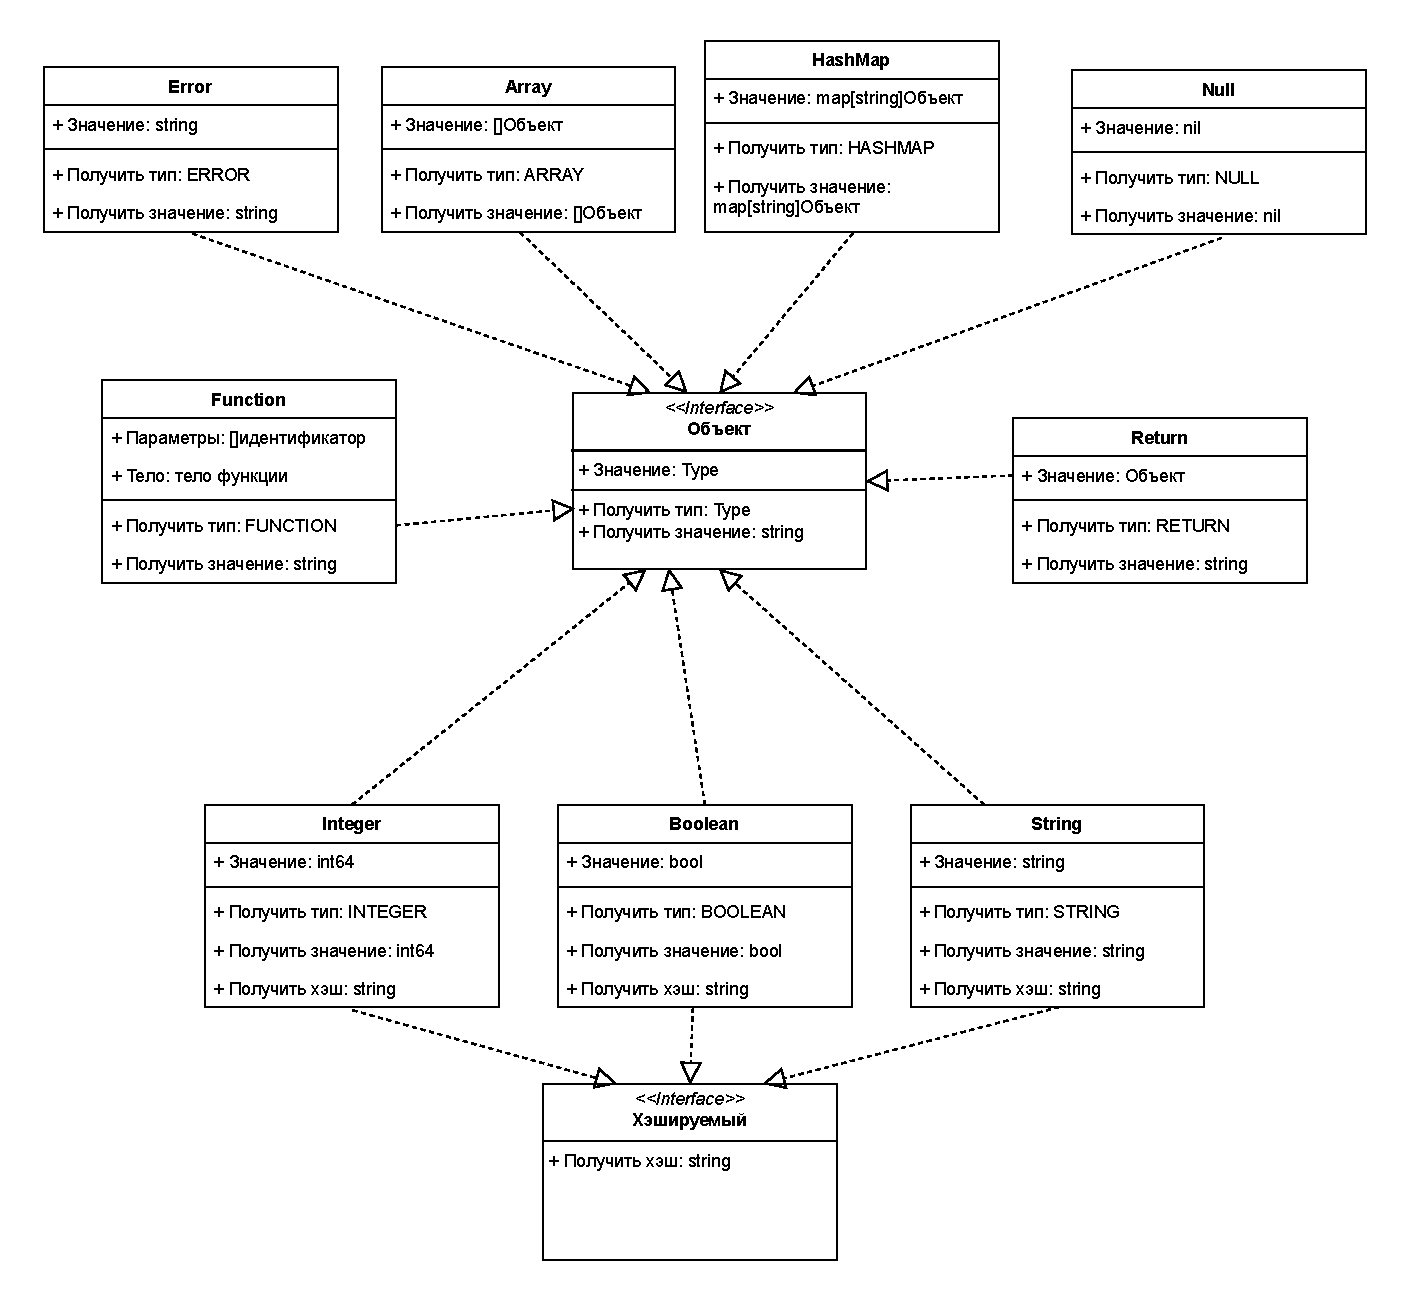
\includegraphics[width=1.0\textwidth]{structures/semantic_analyzer/class_diagram.pdf}
	\caption{Диаграмма классов}
	\label{f:class_diagram}
\end{figure}

В качестве примера работы алгоритма на рисунках~\ref{f:semantic_infix_expr}~-~\ref{f:semantic_index_expr} приведены схемы алгоритмов семантического анализа некоторых выражений.

В данном разделе была выполнена разработка структурных решений и алгоритмов функционирования семантического анализатора.

\begin{figure}[!htp]
	\centering
	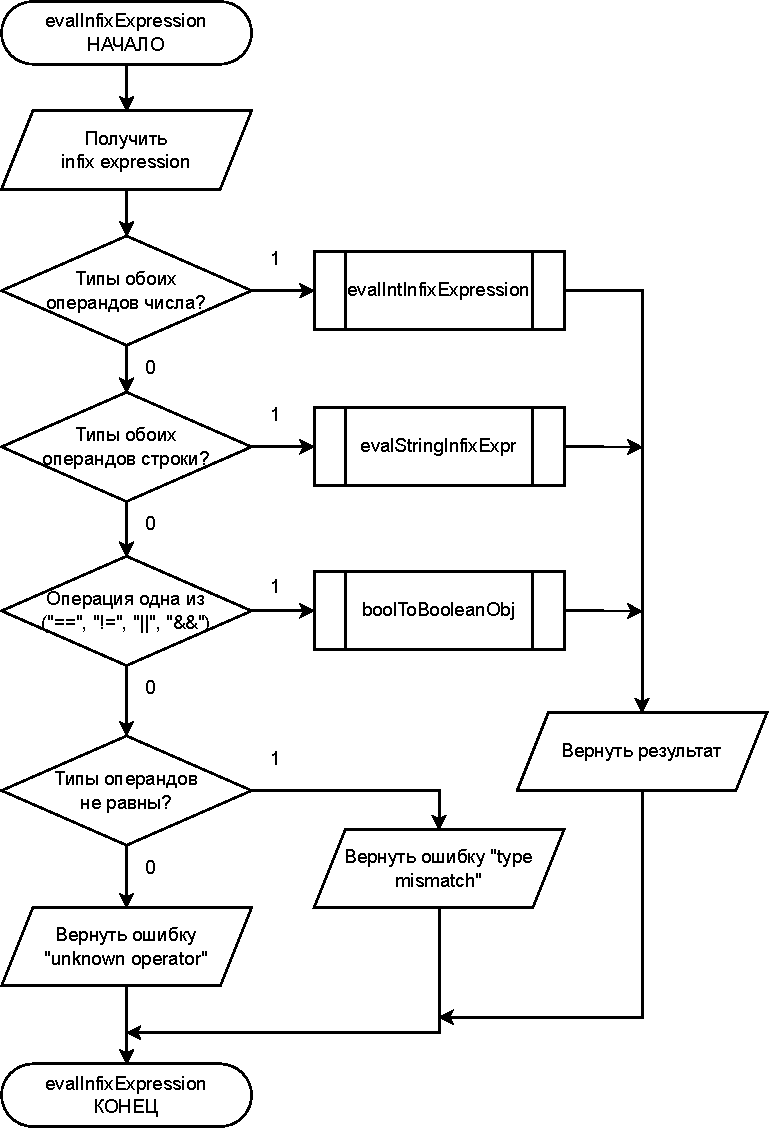
\includegraphics[width=0.9\textwidth]{structures/semantic_analyzer/semantic_infix_expr.pdf}
	\caption{Схема алгоритма «evalInfixExpression»}
	\label{f:semantic_infix_expr}
\end{figure}

\clearpage

\begin{figure}[!htp]
	\centering
	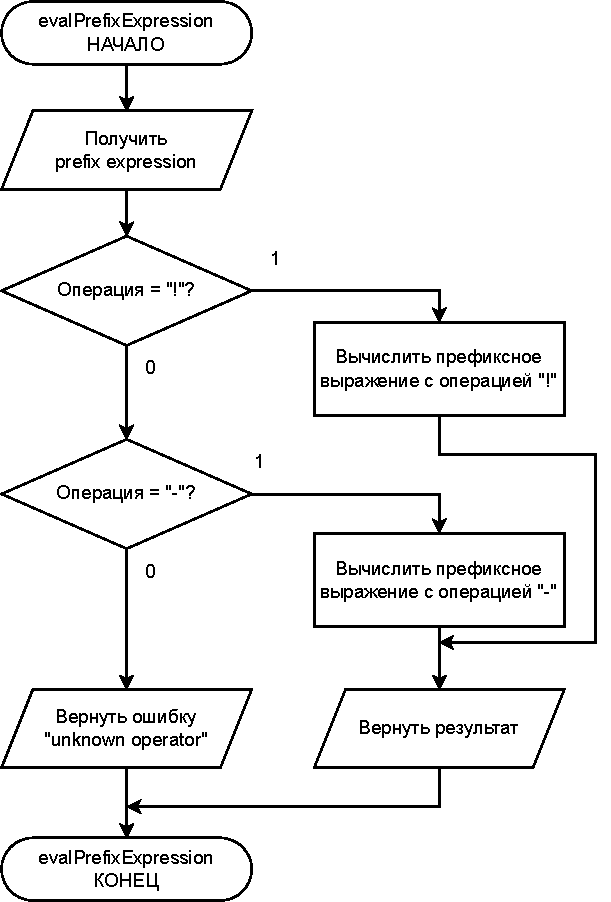
\includegraphics[width=0.9\textwidth]{structures/semantic_analyzer/semantic_prefix_expr.pdf}
	\caption{Схема алгоритма «evalPrefixExpression»}
	\label{f:semantic_prefix_expr}
\end{figure}

\clearpage

\begin{figure}[!htp]
	\centering
	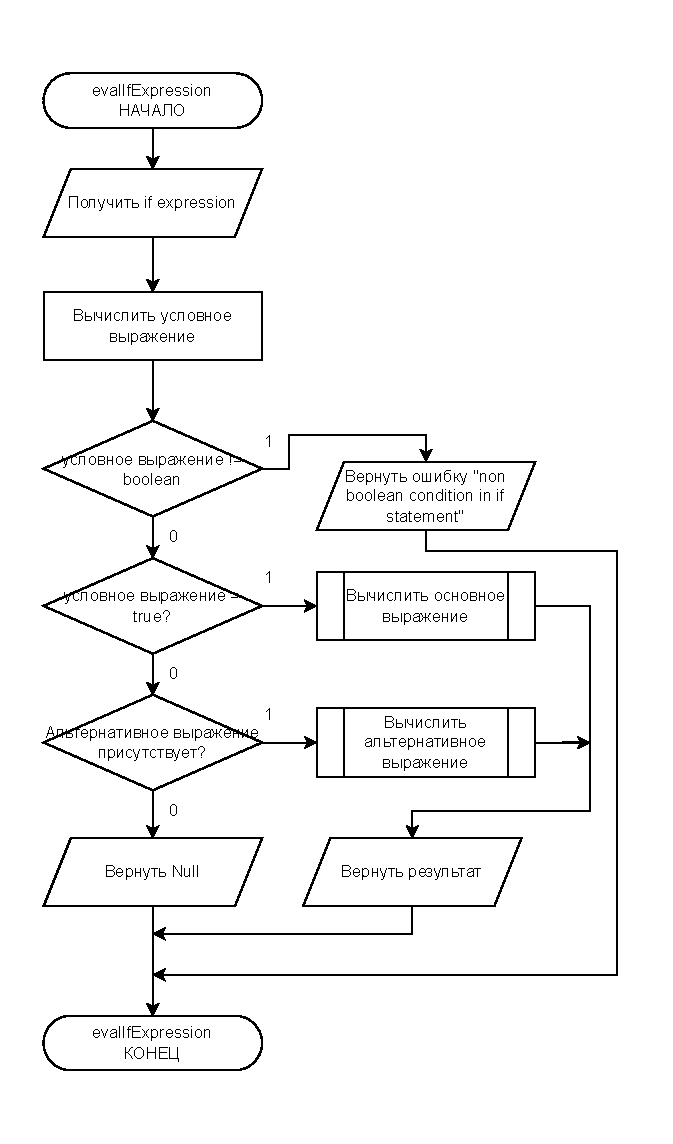
\includegraphics[width=0.75\textwidth]{structures/semantic_analyzer/semantic_if_expr.pdf}
	\caption{Схема алгоритма «evalIfExpression»}
	\label{f:semantic_if_expr}
\end{figure}

\clearpage

\begin{figure}[!htp]
	\centering
	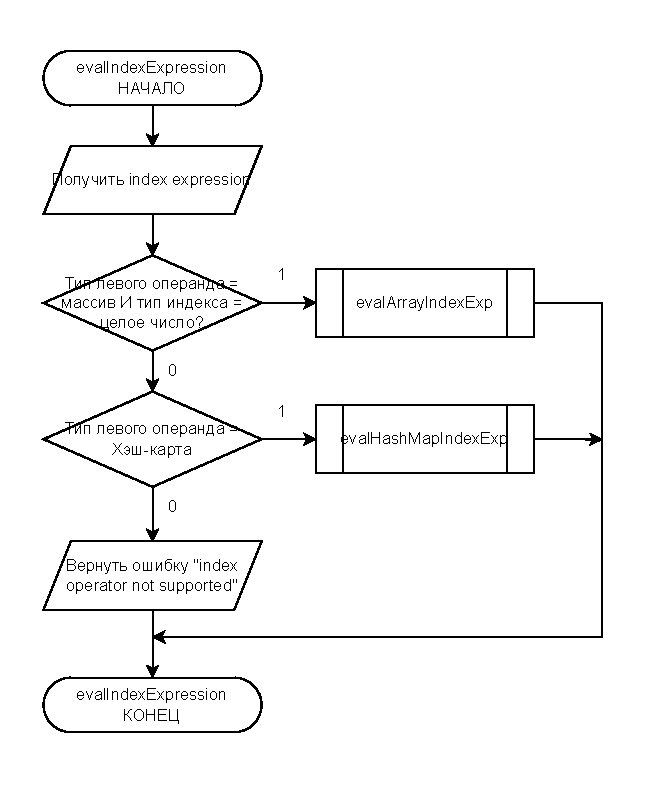
\includegraphics[width=0.75\textwidth]{structures/semantic_analyzer/semantic_index_expr.pdf}
	\caption{Схема алгоритма «evalIndexExpression»}
	\label{f:semantic_index_expr}
\end{figure}